\section{Trading Environment}
We build a customized Open AI Gym environment that has two primary goals. The first objective is to translate domain-specific inputs into state/reward as inputs to the RL model. Most RL models are for general purposes; we need to translate features from the finance market into the observable states, which can be the input to the RL model. 
\par
The second goal is to build the portfolio from the output of the RL model. RL models output action; in our case, it's a continuous space between 0 and 1. We need to build our portfolio from the action.
\par
The trading environment contains few major components, Feature Extractor, Portfolio Builder, Trading System, and the Reward Provider.

\subsection {Feature Extractor}
The Feature Extract extracts features from the market as part of states

\begin{figure}[ht]
  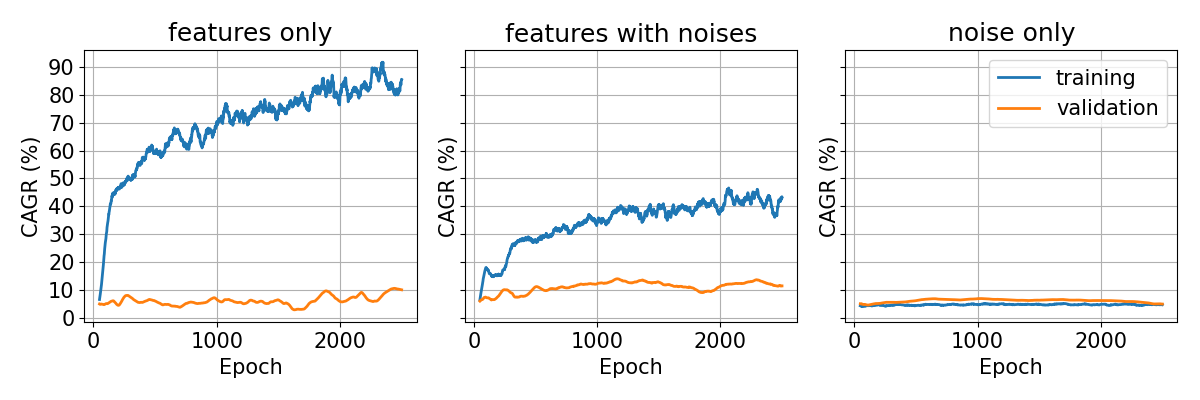
\includegraphics[width=15cm]{images/compare_noise.png}
  \caption{Comparison of states with noise, state without nosie, and nosie only in terms of training/validation CAGR }
  \label{fig:noise_diagram}
\end{figure}

\subsection {Portfolio Builder}
The Portfolio Builder Build the portfolio from investments and actions
\subsection {Trading System}
The Trading System measures performances of the given portfolios
\subsection {Reward Provider}
The Reward Provider provides reward from performances of the portfolio and investor preference